\documentclass[11pt]{article}

% ---------- packages ----------
\usepackage[utf8]{inputenc}
\usepackage[T1]{fontenc}
\usepackage{lmodern}
\usepackage[margin=1in]{geometry}
\usepackage{amsmath,amssymb}
\usepackage{booktabs}
\usepackage{array}
\usepackage{graphicx}
\usepackage{xcolor}
\usepackage{tikz}
\usetikzlibrary{arrows.meta,positioning,fit,backgrounds}
\usepackage{caption}
\usepackage{enumitem}
\usepackage[hidelinks]{hyperref}
\usepackage{microtype}

\captionsetup{font=small,labelfont=bf}
\setlength{\parskip}{0.35em}
\setlength{\emergencystretch}{3em}
\newcommand{\code}[1]{\texttt{\small #1}}

% ---------- title ----------
\title{\bfseries LLM-Enhanced Process-Aware Knowledge Tracing\\
from Student Solution Steps for Concept Deficiency Prediction}
\author{Temesgen\\[2pt]
\normalsize University of Vienna}
\date{June 2026}

\begin{document}
\maketitle

\begin{abstract}
\noindent
Classical knowledge tracing (KT) predicts only whether a student will answer the
next question correctly. The recent \emph{ConceptKT} benchmark reframes the task as
\emph{concept-level deficiency prediction}: given a student's history, predict
\emph{which} of $55$ mathematical concepts they will be deficient in on their next
problem. This is far more useful pedagogically but also far harder---trained KT
models score near zero on it, and only large language models (LLMs), used end-to-end
at inference, reach useful accuracy. This report studies a hybrid that occupies the
gap between these extremes. We use a Gemini LLM \emph{offline}, exactly once per
\emph{past} interaction, as a process \emph{analyzer} that turns each worked
solution into structured signals (missing concepts, error type, a faulty step, a
plain-language process summary), and then train a small, cheap DKT-style LSTM on
those \emph{past-only} features to predict future deficiencies. On the official
MathEDU/ConceptKT split ($3{,}644$ train / $404$ test, $6$ students) and averaged
over five seeds, the offline LLM features raise deficiency macro-F1 over $13$
categories from $24.0\%$ (a correctness-only DKT baseline) to $28.3\%$, recovering
about $60\%$ of the gap to a gold-feature ceiling of $31.1\%$, with both precision
and recall improving. Leakage is made \emph{structural}---enforced by a runtime
assertion with a negative self-test---and the whole pipeline is deterministic and
reproducible offline. The answer to the research question is a qualified yes: in a
genuinely low-resource setting, LLM-derived process signals improve diagnostic KT
over correctness alone.
\end{abstract}

% =====================================================================
\section{Introduction}
% =====================================================================
Knowledge tracing (KT) models a student's evolving knowledge state from a sequence
of learning interactions and predicts future performance. Traditional KT methods
rely on question identifiers, skill labels, and correctness outcomes
\cite{piech2015dkt}. Although effective at predicting the next answer, this setting
discards the student's actual problem-solving \emph{process}, which often contains
richer evidence about misconceptions, partial understanding, and missing
prerequisite concepts than the final answer alone \cite{huang2024remembering}.

A recent line of work moves toward \emph{process-aware} and \emph{text-aware} KT,
showing that student solution processes can be incorporated into KT and that
language models provide useful semantic and reasoning signals for educational
prediction \cite{lee2024lkt,park2025statuskt,ozyurt2024kcqrl}. Building on this, the
\emph{ConceptKT} benchmark \cite{kang2026conceptkt} replaces binary correctness with
\emph{concept-level deficiency prediction}: given a student's history, predict the
specific concepts the student is currently deficient in. This is diagnostically
valuable---it tells a teacher \emph{what to reteach}---but much harder: on ConceptKT,
trained KT baselines are nearly useless at deficiency (the best, OKT, reaches
$1.87\%$ macro-F1), while only an end-to-end LLM reaches $\approx 17\%$
\cite{kang2026conceptkt}.

This report investigates the research question posed in the project proposal:

\begin{quote}\itshape
Can LLM-derived process signals from student solution steps improve concept
deficiency prediction compared with a correctness-only baseline?
\end{quote}

Our central design choice is to use the LLM \emph{not} as an end-to-end predictor
but as an \emph{offline process-analysis module}. The LLM reads each \emph{past}
solution exactly once and emits structured pedagogical signals; a small trained
sequence model then consumes those signals to predict future deficiencies. This
keeps the LLM where it is strong (reading one solution) and a tiny LSTM where data
is scarce (only six students). We make three contributions:

\begin{enumerate}[leftmargin=1.4em,itemsep=2pt,topsep=2pt]
\item A complete, reproducible hybrid pipeline---offline Gemini analyzer with a
disk cache, leakage-safe sequence construction, and a two-head DKT-style LSTM---for
concept deficiency prediction on MathEDU/ConceptKT.
\item A clean three-arm experiment (correctness-only baseline, LLM process-aware,
and a \emph{gold-feature upper bound}) that isolates the value of the LLM features
and quantifies the headroom a better analyzer could still capture.
\item An emphasis on methodological rigor: leakage is enforced structurally and
tested negatively, class imbalance is handled explicitly, results are reported as
mean\,$\pm$\,std over five seeds, and the entire run is reproducible offline.
\end{enumerate}

Across five seeds, the offline LLM features improve deficiency macro-F1@13 by
$+4.3$ points over the baseline and recover $\sim\!60\%$ of the gap to gold
features. We report these results honestly: with six students and $59$ positive test
labels the decimals are noisy, so the robust finding is the \emph{ordering}
A\,$<$\,B\,$<$\,C, not the exact values.

% =====================================================================
\section{Related Work}
% =====================================================================
\paragraph{Deep and interpretable KT.}
Deep Knowledge Tracing introduced neural sequence modeling to KT and established the
modern formulation of predicting performance from interaction histories
\cite{piech2015dkt}. Subsequent models (DKVMN, SAKT, GKT, and others) refined the
sequence backbone but still consume only correctness and skill signals. A more
recent strand argues that \emph{remembering is not applying} and models the
problem-solving process itself for interpretability \cite{huang2024remembering}.
Our work shares that motivation but targets the harder \emph{deficiency} output
rather than correctness.

\paragraph{Text-aware and LM-enhanced KT.}
Language-model representations of question and concept text can improve KT,
especially where semantics matter and for cold-start items \cite{lee2024lkt}.
KCQRL shows that an LLM can annotate knowledge concepts at the \emph{solution-step}
level and that contrastive, concept-aligned embeddings consistently improve $15$ KT
models across two large datasets \cite{ozyurt2024kcqrl}. This directly justifies two
of our choices: deriving concept/process features from an LLM, and embedding the
analyzer's free-text summary with a frozen sentence encoder.

\paragraph{Process signals as intermediate features.}
Closest in spirit, StatusKT/KT-PSP uses a teacher--student--teacher three-stage LLM
pipeline to extract mathematical-proficiency signals from problem-solving processes
and feeds them, as intermediate signals, into existing KT backbones, improving both
accuracy and interpretability over correctness-only KT \cite{park2025statuskt}. Our
prototype follows the same blueprint---\emph{LLM as an offline analyzer producing
structured signals that a trained KT model consumes}---but in a deliberately minimal,
low-resource form, and it measures the contribution of those signals against an
explicit gold-feature ceiling.

\paragraph{The benchmark.}
ConceptKT \cite{kang2026conceptkt} defines our task, label space, and split. It is
built on MathEDU \cite{hsu2026mathedu}, a corpus of authentic student mathematical
solution processes with correctness labels, teacher error annotations, and feedback.
ConceptKT runs the LLM \emph{end-to-end} (in-context learning over selected response
histories); the trained KT baselines it reports use correctness only. Our hybrid
sits between these two regimes (Table~\ref{tab:positioning}).

\begin{table}[t]
\centering
\caption{Where this work sits. The LLM is used neither purely end-to-end nor not at
all, but \emph{offline}, once per past interaction, as a feature extractor for a
small trained model.}
\label{tab:positioning}
\small
\begin{tabular}{@{}lccc@{}}
\toprule
& \textbf{Trained KT} & \textbf{End-to-end LLM} & \textbf{This work (hybrid)}\\
\midrule
LLM role            & none            & predictor (inference) & offline analyzer\\
Sequence model      & yes             & no                    & yes (small LSTM)\\
Inference cost      & low             & high                  & low\\
Deficiency quality  & very low        & moderate              & between baseline \& gold\\
\bottomrule
\end{tabular}
\end{table}

% =====================================================================
\section{Data}
% =====================================================================
We use two public repositories from the NYCU NLP Lab that describe the \emph{same}
$4{,}048$ interactions from $6$ students, seen from two angles.

\textbf{MathEDU}~\cite{hsu2026mathedu} is the \emph{process} side: each record holds
a MathQA problem \code{id}, the \code{student\_id}, the student's final answer, the
worked \code{student\_process} (in \LaTeX), a correctness label, and---when
incorrect---a \code{teacher\_review} with an error type and an error equation.
\textbf{ConceptKT}~\cite{kang2026conceptkt} is the \emph{label} side: for every
record it provides the gold \code{associated\_concepts} (the concepts a problem
requires) and \code{missing\_concepts} (the concepts a student failed to apply;
empty when correct), drawn from a fixed taxonomy of $55$ concepts grouped into $13$
categories. It also ships the official chronological $90/10$ split
($3{,}644$ train / $404$ test).

\paragraph{Joining the two sources.}
The datasets are merged record-by-record with ConceptKT as the ``spine,'' because
it owns the chronological order, the official split, and the gold labels; MathEDU's
process fields attach onto it. We join on the composite key
\code{(id, student\_id)}, which gives $100\%$ coverage ($4{,}048/4{,}048$);
\code{id} alone is not unique because several students attempt the same MathQA
problem. Two edge cases are handled so the split reproduces exactly: ConceptKT
contains two duplicate \code{(id, student\_id)} rows (a re-attempt), which we tag by
taking the chronological \emph{tail} for the official test set, and MathEDU's eight
raw error strings are normalized onto a six-way enum
(e.g.\ \emph{Arithmetical/Algebraic/Measurement error} $\rightarrow$
\code{calculation\_error}). A subtle but important point is that the chronological
order is the \emph{position within ConceptKT}, grouped by student---\code{id} is a
MathQA problem identifier, not a timestamp, so the data must never be sorted by it.

\paragraph{Key statistics that shaped the design.}
Table~\ref{tab:data} summarizes the corpus. Three facts drove several decisions.
First, the data is \emph{heavily imbalanced}: $75.3\%$ of answers are correct, and
only $463$ records ($11.4\%$) carry a non-empty deficiency target. Second, the
signal is \emph{sparse at test time}: the $404$ test targets contain just $59$
positive concept labels in total, which makes macro-F1 noisy and motivates
imbalance-aware loss, threshold tuning, and reporting at the coarser $13$-category
level. Third, MathEDU carries \emph{no question text} (its \code{id} maps to MathQA),
so the analyzer must work from the student's solution alone; this does not affect the
deficiency \emph{targets}, which come from ConceptKT gold.

\begin{table}[t]
\centering
\caption{MathEDU/ConceptKT corpus statistics (from \code{src/eda.py}).}
\label{tab:data}
\small
\begin{tabular}{@{}lr@{\hspace{2.2em}}lr@{}}
\toprule
\textbf{Quantity} & \textbf{Value} & \textbf{Quantity} & \textbf{Value}\\
\midrule
Interactions            & $4{,}048$ & Concepts / categories      & $55$ / $13$\\
Students                & $6$       & Correct answers            & $3{,}050$ ($75.3\%$)\\
Train / test (official) & $3{,}644$ / $404$ & Wrong answers      & $998$ ($24.7\%$)\\
Records with gold deficiency & $463$ ($11.4\%$) & Conceptual deficiency & $722$ ($17.8\%$)\\
Test positive concept labels & $59$  & Careless errors            & $276$ ($6.8\%$)\\
\bottomrule
\end{tabular}
\end{table}

% =====================================================================
\section{Method}
% =====================================================================
The pipeline (Figure~\ref{fig:pipeline}) turns each raw record into structured LLM
features, encodes them numerically, assembles one leakage-safe sequence per student,
and trains a two-head LSTM whose deficiency head is masked to the target question's
associated concepts.

\begin{figure}[t]
\centering
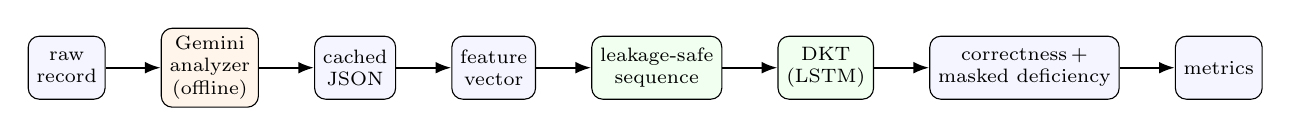
\begin{tikzpicture}[
  node distance=6mm and 7mm,
  box/.style={draw,rounded corners,align=center,inner sep=3pt,font=\scriptsize,
              minimum height=8mm,fill=blue!4},
  arr/.style={-{Latex[length=2mm]},thick}
]
\node[box] (raw) {raw\\record};
\node[box,right=of raw,fill=orange!8] (llm) {Gemini\\analyzer\\(offline)};
\node[box,right=of llm] (cache) {cached\\JSON};
\node[box,right=of cache] (feat) {feature\\vector};
\node[box,right=of feat,fill=green!6] (seq) {leakage-safe\\sequence};
\node[box,right=of seq,fill=green!6] (dkt) {DKT\\(LSTM)};
\node[box,right=of dkt] (heads) {correctness\,+\\masked deficiency};
\node[box,right=of heads] (met) {metrics};
\draw[arr] (raw)--(llm); \draw[arr] (llm)--(cache); \draw[arr] (cache)--(feat);
\draw[arr] (feat)--(seq); \draw[arr] (seq)--(dkt); \draw[arr] (dkt)--(heads);
\draw[arr] (heads)--(met);
\end{tikzpicture}
\caption{End-to-end data flow. The LLM is consulted once per past interaction and
its output is cached; everything downstream is a small, deterministic, trained model.}
\label{fig:pipeline}
\end{figure}

\subsection{Offline LLM process analyzer}
For each interaction the analyzer (\code{src/llm\_analyzer.py}) issues a single
Gemini call (model \code{gemini-3.1-flash-lite}, read from an environment variable
so models can be swapped without code changes) that \emph{describes what already
happened} in the solution and returns a fixed JSON object---
\code{associated\_concepts}, \code{missing\_concepts}, a six-way
\code{error\_type}, a \code{faulty\_step}, \code{partial\_understanding}, and a
one-to-two sentence \code{process\_summary}---enforced by a Pydantic response schema.
Several design choices make this component reliable and cheap:

\begin{itemize}[leftmargin=1.3em,itemsep=2pt,topsep=2pt]
\item \textbf{Determinism.} \code{temperature\,=\,0} plus a JSON schema yields
reproducible, always-parseable output.
\item \textbf{Caching.} Each result is stored on disk under a key of
\code{sha256(prompt\_version\,|\,model\,|\,prompt)}, so re-running the pipeline makes
\emph{zero} API calls and byte-identical solutions share a file. The initial
extraction made $3{,}882$ live API calls with \emph{zero failures}, producing
$3{,}962$ unique cached analyses that cover all $4{,}048$ interactions, at a cost
well under \$5.
\item \textbf{Pinned behavior and sanitation.} A system instruction forces the model
to choose concepts only from the fixed $55$ (exact strings) and to set
\code{missing\_concepts}\,$=\![\,]$, \code{error\_type}\,$=$\,\code{none} for correct
answers; a post-hoc sanitizer drops any hallucinated concept and re-enforces these
invariants so a misbehaving model cannot corrupt the label space.
\item \textbf{Split failure policy.} Malformed model output is retried once and then
cached as a null placeholder (a genuine per-record failure), whereas API/auth errors
are retried once and then \emph{raised, never cached}, so a bad key cannot poison the
cache.
\end{itemize}

\subsection{Feature encoding}
Each interaction is encoded (\code{src/features.py}) into the components in
Table~\ref{tab:features}. The error type is emitted as an integer id and turned into
a learned $8$-dimensional embedding \emph{inside} the model, since a small
categorical signal is best learned rather than hand-coded. The process summary is
embedded with a \emph{frozen} \code{all-MiniLM-L6-v2} sentence transformer
\cite{reimers2019sbert}: with only six students there is no data to fine-tune an
encoder, so it is used purely as a fixed semantic featurizer, in the spirit of
KCQRL \cite{ozyurt2024kcqrl}.

\begin{table}[t]
\centering
\caption{Per-interaction feature components and the arms that use them (Sec.~4.4).
``Assoc.'' concepts are a known property of the question and are also used as the
output mask.}
\label{tab:features}
\small
\begin{tabular}{@{}llcl@{}}
\toprule
\textbf{Component} & \textbf{Dim} & \textbf{Used by} & \textbf{Source}\\
\midrule
\code{assoc\_multihot}        & $55$  & A,\,B,\,C & gold associated concepts (+\,mask)\\
\code{correct}                & $1$   & A,\,B,\,C & grading\\
\code{llm\_missing\_multihot} & $55$  & B         & analyzer \code{missing\_concepts}\\
\code{llm\_error\_type}       & emb.  & B         & analyzer \code{error\_type}\\
\code{summary\_embed}         & $384$ & B         & frozen ST(\code{process\_summary})\\
\code{gold\_missing\_multihot}& $55$  & C\,(+target) & gold \code{missing\_concepts}\\
\code{gold\_error\_type}      & emb.  & C         & gold (normalized) error type\\
\bottomrule
\end{tabular}
\end{table}

\subsection{Leakage-safe sequence model}
We build one chronological sequence per student (\code{src/dataset.py}). At step $i$
the model sees the features of interaction $i$ and predicts interaction $i\!+\!1$:
the hidden state of the LSTM after consuming steps $0\ldots i$ produces the
prediction for the $(i\!+\!1)$-th target, so a target's own features are never in the
window used to predict it.

The backbone (\code{src/model.py}) is a deliberately basic single-layer LSTM
(hidden size $64$, dropout $0.4$) with two prediction heads applied to the
next-step hidden state:
\begin{itemize}[leftmargin=1.3em,itemsep=2pt,topsep=2pt]
\item a \textbf{correctness head} (one logit, trained with binary cross-entropy), and
\item a \textbf{deficiency head} ($55$ logits). Because $\text{missing}\subseteq
\text{associated}$, logits for concepts \emph{not} associated with the target
question are masked to $-10^{9}$ before loss and prediction. This removes $\sim\!53$
of $55$ trivial negatives per example and focuses learning on the real candidates.
\end{itemize}
The masked deficiency entries are trained with \emph{focal} binary cross-entropy
(focusing parameter $\gamma\!=\!2$) \cite{lin2017focal}, which down-weights the easy
negatives that dominate this head; correctness uses plain BCE. The model is small on
purpose---with six students, anything larger memorizes.

\subsection{Three experimental arms}
All arms share the \emph{same} model class and training code; only the per-step input
changes, which isolates the effect of the features.
\begin{description}[leftmargin=2.2em,itemsep=2pt,topsep=2pt,style=nextline]
\item[\textnormal{\textbf{Arm A} (baseline)}] \code{assoc\_multihot\,+\,correct} ---
a correctness-only DKT baseline.
\item[\textnormal{\textbf{Arm B} (process-aware)}] Arm A $+$ the LLM features
(\code{llm\_missing\_multihot}, \code{summary\_embed}, learned error embedding) ---
the system under test.
\item[\textnormal{\textbf{Arm C} (gold ceiling)}] Arm A $+$ \emph{gold} past missing
concepts and gold error type --- the upper bound with perfect features.
\end{description}
B\,$-$\,A measures the value of the LLM; C\,$-$\,B measures how much a better analyzer
could still add. A useful sanity property follows from this design: arms A and C never
touch the LLM, so they are byte-identical between a synthetic ``mock'' run and the
real Gemini run---only arm B changes when synthetic features are swapped for real ones,
exactly as it should.

\subsection{Leakage prevention is structural, not a convention}
\label{sec:leakage}
The hard constraint is that the analyzer and the model may only ever see interactions
\emph{before} the target, and the analyzer must never read the target's own solution.
We make this structural in five ways: (i) the analyzer only ever receives one
already-completed interaction at a time; (ii) the model is strictly causal by
construction (Sec.~4.3); (iii) gold \code{missing\_concepts} are the \emph{target} and
are used as an \emph{input} only by arm C and only for past steps; (iv) a runtime
assertion (\code{\_assert\_no\_leakage}) runs on \emph{every} built sequence and
checks that each target's global index is strictly greater than every input index used
to predict it; and (v) a \emph{negative test} deliberately injects a target into its
own history and confirms the assertion \emph{fires}---so we know the guard works, not
merely that it exists. Using a question's associated concepts as an input feature and
as the output mask is \emph{not} leakage, because they are a known property of the
problem the moment it is shown.

% =====================================================================
\section{Experimental Setup}
% =====================================================================
\paragraph{Protocol.}
We use the official ConceptKT chronological split ($3{,}644$ train / $404$ test). For
early stopping we carve a validation set from the last $10\%$ of each student's
\emph{train} history (still strictly before any test target). Each
$(\text{arm},\text{seed})$ is trained with Adam (learning rate $10^{-3}$), up to
$60$ epochs with early stopping (patience $8$) on validation loss. The feature store
(including summary embeddings) is built \emph{once} and reused across all arms and
seeds. We report mean\,$\pm$\,std over five seeds $\{0,\dots,4\}$.

\paragraph{Threshold tuning.}
The deficiency head is a heavily imbalanced multi-label classifier; with a fixed
$0.5$ threshold it predicts all-negative and macro-F1 collapses to $0$, hiding any
difference between arms. After training, we therefore search a small grid
($0.10\ldots0.50$) and pick the decision threshold that maximizes \emph{validation}
macro-F1@13, then apply it once to the test set. The threshold is chosen on validation,
never on test, so the comparison is honest.

\paragraph{Metrics.}
Correctness is scored with accuracy and AUC. Deficiency is scored with macro
precision/recall/F1 at \emph{both} the $55$-concept level (fine, sparse) and the
$13$-category level (obtained by OR-ing each category's concepts; coarser and more
stable given the sparsity). We also keep per-category F1 for the error analysis.

\paragraph{Reproducibility.}
With five fixed seeds, the official split, and a warm analyzer cache, the training
command makes \emph{zero} API calls and reproduces \code{results/metrics.json}
bit-for-bit. A deterministic \code{pytest} suite of $45$ tests (no live API) guards
the load-bearing logic: the concept/error taxonomy, the per-arm feature layout, the
leakage assertion (tested to fire), analyzer caching and hallucination sanitation,
the metrics, and the model's forward/mask/loss shapes.

% =====================================================================
\section{Results}
% =====================================================================
\subsection{Analyzer validation}
Before trusting the analyzer on all $4{,}048$ interactions, we validated it against
the gold teacher annotations on $20$ incorrect records. It agreed with the gold error
type on \textbf{$15/20$ ($75\%$)} of cases, with many exact \code{faulty\_step}
matches; the disagreements cluster on the genuinely fuzzy
\code{calculation\_error}\,$\leftrightarrow$\,\code{wrong\_operation\_or\_concept}
boundary. This was judged sufficient to proceed.

\subsection{Main result: do the LLM features help?}
Table~\ref{tab:main} reports the headline numbers. The ordering is consistent and
monotone on every deficiency metric: \textbf{A\,$<$\,B\,$<$\,C}.

\begin{table}[t]
\centering
\caption{Deficiency prediction on the official test set, mean\,$\pm$\,std over five
seeds. Correctness accuracy is flat because the head is dominated by the $75\%$
base rate of correct answers; \emph{deficiency} is where the process features add
value.}
\label{tab:main}
\small
\begin{tabular}{@{}lcccccc@{}}
\toprule
\textbf{Arm} & \textbf{Acc.} & \textbf{AUC} &
\textbf{F1@55} & \textbf{F1@13} & \textbf{P@13} & \textbf{R@13}\\
\midrule
A --- correctness-only      & $71.78$ & $0.59$ & $10.28$ & $24.04$ & $19.29$ & $39.49$\\
\textbf{B --- process-aware}& $71.78$ & $0.59$ & $\mathbf{12.24}$ & $\mathbf{28.31}$ & $25.16$ & $47.24$\\
C --- gold ceiling          & $71.78$ & $0.59$ & $13.36$ & $31.10$ & $28.78$ & $45.60$\\
\midrule
\multicolumn{2}{@{}l}{$\pm$\,std on F1@13} & & & \multicolumn{3}{l}{A:\,$\pm4.18$\quad B:\,$\pm4.73$\quad C:\,$\pm1.46$}\\
\bottomrule
\end{tabular}
\end{table}

Three observations follow.
\textbf{(1) The LLM features help.} Arm B beats arm A by $+4.3$ points of
macro-F1@13 ($24.04\!\rightarrow\!28.31$) and $+2.0$ points at the concept level
($10.28\!\rightarrow\!12.24$). The gain shows up in \emph{both} precision
($19.3\!\rightarrow\!25.2$) and recall ($39.5\!\rightarrow\!47.2$), so it is not a
threshold artifact.
\textbf{(2) They recover most of the gap to gold.} The full headroom A\,$\rightarrow$\,C
is $7.1$ points ($24.04\!\rightarrow\!31.10$); arm B reaches $28.31$, i.e.\
$\approx\!60\%$ of the way to perfect features. The remaining $2.8$ points
(B\,$\rightarrow$\,C) is what a sharper analyzer could still contribute.
\textbf{(3) Correctness is flat at $71.78\%$ across all arms.} The correctness head is
dominated by the base rate of correct answers; process features are simply not where
correctness gains come from---deficiency is the interesting signal, as ConceptKT also
found \cite{kang2026conceptkt}.

\subsection{Error analysis: where the process features help}
Table~\ref{tab:erroranalysis} breaks the B\,$-$\,A difference down by category. The
process features help multi-step and word-problem topics most---\emph{Sequences \&
Series} ($+0.35$), \emph{Physics} ($+0.12$), and \emph{Statistics \& Probability}
($+0.10$)---where the LLM's reading of a worked solution disambiguates conceptual
errors that raw correctness cannot. A few categories regress slightly
(\emph{Polynomials} $-0.07$, \emph{Finance} $-0.03$, \emph{Geometry} $-0.02$),
consistent with added feature noise on topics where correctness was already a decent
proxy. Across all $13$ categories, six improve, four are unchanged, and three regress.

\begin{table}[t]
\centering
\caption{Per-category deficiency F1 (mean over seeds), arm~B minus arm~A. Positive
means the offline LLM features helped that category. Categories with no test
positives are omitted from the highlights.}
\label{tab:erroranalysis}
\small
\begin{tabular}{@{}lccc@{}}
\toprule
\textbf{Category} & \textbf{A} & \textbf{B} & \textbf{$\Delta$ (B$-$A)}\\
\midrule
Sequences and Series        & $0.114$ & $0.460$ & $+0.346$\\
Physics                     & $0.114$ & $0.237$ & $+0.123$\\
Statistics and Probability  & $0.000$ & $0.096$ & $+0.096$\\
Ratio and Proportion        & $0.000$ & $0.053$ & $+0.053$\\
Set Theory                  & $0.133$ & $0.178$ & $+0.044$\\
Prime Numbers               & $0.391$ & $0.397$ & $+0.006$\\
Geometry                    & $0.533$ & $0.515$ & $-0.019$\\
Finance                     & $0.481$ & $0.454$ & $-0.027$\\
Polynomials                 & $0.500$ & $0.433$ & $-0.067$\\
\bottomrule
\end{tabular}
\end{table}

\subsection{Context: the ConceptKT paper baselines}
Table~\ref{tab:context} reproduces the ConceptKT paper's reported numbers
\cite{kang2026conceptkt}. Two things stand out. First, trained KT models predict
correctness reasonably ($63$--$69\%$) but are essentially useless at deficiency
(OKT: $1.87\%$ macro-F1); only an end-to-end LLM reaches $\approx\!17\%$. Second,
\emph{this is context, not a head-to-head}: although we use the paper's exact split
and gold labels, our modeling setup differs fundamentally (a small DKT on
\emph{past-only} offline features vs.\ their end-to-end in-context LLM), and our
$13$-category F1 is a coarser metric than their $55$-concept macro-F1. The comparison
that this report controls cleanly is the internal A/B/C contrast of
Table~\ref{tab:main}.

\begin{table}[t]
\centering
\caption{ConceptKT paper baselines \cite{kang2026conceptkt} (context only --- a
different setup, not directly comparable to Table~\ref{tab:main}).}
\label{tab:context}
\small
\begin{tabular}{@{}lcc@{}}
\toprule
\textbf{Method} & \textbf{Correctness acc.} & \textbf{Deficiency macro-F1}\\
\midrule
DKT                       & $64.80$ & ---\\
DKVMN                     & $63.10$ & ---\\
GKT                       & $63.20$ & ---\\
SAKT                      & $66.46$ & ---\\
OKT                       & $69.25$ & $1.87$\\
Best LLM (DeepSeek-R1, ICL) & $71.02$ & $17.40$\\
\bottomrule
\end{tabular}
\end{table}

% =====================================================================
\section{Discussion}
% =====================================================================
\paragraph{Answering the research question.}
The evidence supports a qualified ``yes.'' Offline LLM-derived process signals
improve concept deficiency prediction over a correctness-only baseline---$+4.3$ points
of macro-F1@13, with gains in both precision and recall, and a clean monotone
ordering A\,$<$\,B\,$<$\,C across seeds and granularities. Crucially, the improvement
comes from features extracted \emph{once, offline}, by reading each past solution; the
trained model that consumes them is tiny and cheap at inference. This is precisely the
``LLM as interpretable process analyzer rather than end-to-end predictor'' regime the
proposal set out to test.

\paragraph{Why the gold ceiling matters.}
Arm C is not just a baseline but a measuring stick. By recovering $\sim\!60\%$ of the
A\,$\rightarrow$\,C gap, arm B shows that the offline analyzer already captures most of
the available signal in these features, while the remaining $40\%$ ($2.8$ points)
quantifies---rather than merely asserts---the value of a sharper analyzer. The
$75\%$ analyzer--gold agreement on error type is consistent with this residual gap.

\paragraph{Honesty about noise.}
With six students and $59$ positive test labels, the per-seed F1@13 varies by several
points (note the $\pm4$ std on arms A and B). The robust claim is therefore the
\emph{ordering}, not the exact decimals; arm C's much tighter spread ($\pm1.46$) is
itself evidence that cleaner features both raise and stabilize performance. We also
stress that the paper baselines in Table~\ref{tab:context} are context only.

% =====================================================================
\section{Limitations and Future Work}
% =====================================================================
\textbf{Limitations.} The dataset is tiny (six students, $59$ positive test labels),
so metrics are noisy and conclusions are directional rather than precise. MathEDU
provides no question text, so the analyzer reads only the student's solution (the
deficiency \emph{targets} are unaffected, being gold). We use a single prompt, a
single model, and a single LLM, with no prompt- or model-sensitivity study, and the
backbone is a basic LSTM rather than a state-of-the-art KT model.

\textbf{Future work}, in rough order of value: (i)~swap the LSTM for a stronger
backbone (AKT\slash SAKT\slash GKT\slash DKVMN) via pyKT \cite{liu2022pykt} while keeping the same
feature vector; (ii)~replace feature concatenation with a learned \emph{gated fusion}
so the model can down-weight noisy analyzer features per step; (iii)~adopt
leave-one-student-out evaluation, a more honest generalization test than the
chronological split given six students; (iv)~run a prompt-sensitivity study, since the
offline-feature approach is only useful if it is stable; (v)~join real question text
via MathQA and re-extract; and (vi)~calibrate per-concept thresholds instead of a
single global one.

% =====================================================================
\section{Conclusion}
% =====================================================================
We presented a minimal, reproducible hybrid for concept deficiency prediction that
uses a Gemini LLM offline---once per past interaction---as a structured process
analyzer, and trains a small leakage-safe DKT-style LSTM on the resulting
past-only features. On the official MathEDU/ConceptKT split, the offline LLM features
raise deficiency macro-F1@13 from $24.0\%$ to $28.3\%$ over a correctness-only
baseline, recovering about $60\%$ of the gap to a gold-feature ceiling of $31.1\%$,
with both precision and recall improving. The result is delivered with structural
leakage guarantees, explicit imbalance handling, five-seed reporting, and full offline
reproducibility. In a genuinely low-resource diagnostic-KT setting, transforming
student solution steps into structured pedagogical signals with an offline LLM is a
practical and effective way to improve concept deficiency prediction.

% =====================================================================
\begin{thebibliography}{99}
\setlength{\itemsep}{2pt}

\bibitem{piech2015dkt}
C.~Piech, J.~Bassen, J.~Huang, S.~Ganguli, M.~Sahami, L.~J.~Guibas, and
J.~Sohl-Dickstein, ``Deep Knowledge Tracing,'' in \emph{Advances in Neural
Information Processing Systems (NeurIPS)}, 2015.

\bibitem{huang2024remembering}
T.~Huang, X.~Ou, H.~Yang, Z.~Long, and C.~Xing, ``Remembering is Not Applying:
Interpretable Knowledge Tracing for Problem-Solving Processes,'' in \emph{Proc.\ 32nd
ACM Int.\ Conf.\ on Multimedia (MM)}, 2024, doi:10.1145/3664647.3681049.

\bibitem{lee2024lkt}
U.~Lee, J.~Bae, D.~Kim, S.~Lee, J.~Park, T.~Ahn, G.~Lee, D.~Stratton, and H.~Kim,
``Language Model Can Do Knowledge Tracing: Simple but Effective Method to Integrate
Language Model and Knowledge Tracing Task,'' \emph{arXiv preprint arXiv:2406.02893},
2024.

\bibitem{hsu2026mathedu}
W.-L.~Hsu, Y.-C.~Tang, and A.-Z.~Yen, ``MathEDU: Feedback Generation on
Problem-Solving Processes for Mathematical Learning Support,'' in \emph{Proc.\ 19th
Conf.\ of the European Chapter of the Association for Computational Linguistics
(EACL)}, 2026.

\bibitem{kang2026conceptkt}
Y.-C.~Kang, Y.-C.~Tang, and A.-Z.~Yen, ``ConceptKT: A Benchmark for Concept-Level
Deficiency Prediction in Knowledge Tracing,'' \emph{arXiv preprint arXiv:2603.24073},
2026.

\bibitem{park2025statuskt}
J.~Park, S.~Kang, J.~Park, J.~Kim, J.~Shin, S.~Park, and Y.~Yu, ``Tracing
Mathematical Proficiency Through Problem-Solving Processes,'' \emph{arXiv preprint
arXiv:2512.00311}, 2025.

\bibitem{ozyurt2024kcqrl}
Y.~Ozyurt, S.~Feuerriegel, and M.~Sachan, ``Automated Knowledge Concept Annotation
and Question Representation Learning for Knowledge Tracing,'' \emph{arXiv preprint
arXiv:2410.01727}, 2024.

\bibitem{reimers2019sbert}
N.~Reimers and I.~Gurevych, ``Sentence-BERT: Sentence Embeddings using Siamese
BERT-Networks,'' in \emph{Proc.\ EMNLP-IJCNLP}, 2019.

\bibitem{lin2017focal}
T.-Y.~Lin, P.~Goyal, R.~Girshick, K.~He, and P.~Doll\'ar, ``Focal Loss for Dense
Object Detection,'' in \emph{Proc.\ IEEE Int.\ Conf.\ on Computer Vision (ICCV)},
2017.

\bibitem{liu2022pykt}
Z.~Liu, Q.~Liu, J.~Chen, S.~Huang, B.~Gao, W.~Luo, and J.~Weng, ``pyKT: A Python
Library to Benchmark Deep Learning based Knowledge Tracing Models,'' in \emph{NeurIPS
Datasets and Benchmarks Track}, 2022.

\end{thebibliography}

\end{document}
